\section{Future Work}
\indent The results and process of this study have lead to theories of possible improvements, newly discovered directions to further advance the study, and promising interesting directions.\\
\indent The possible steps to move toward to improve the study take place in the process of frame preparation involving noise reduction. The noise being addressed is any portion of the object in the frame that isn't clearly perceived by the boolean image 
multiplication as seen in Figure 3. 

\begin{figure}[ht]
	\center 
	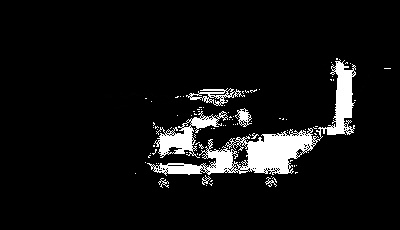
\includegraphics[height = 5cm]{Heli_Noise}
	\caption[Noisy Aerial Manmade Object Profile]{Aerial Manmade Object Profile from Rotorcraft Video Sample: 3 (Noise produced from object contrast during thresholding process)}
\end{figure}

Further clarification of noise include inaccuracies in complete profiles of aerial objects. This noise is caused by high contrast within the object due to the suns reflection, the inability to actively change the threshold in which the binary segmentation occurs, and the inability to automatically center the aerial object from one time interval to the next (more accurate overlay for boolean image multiplication) within the frame (full frame or selected area). The introduction of histogram equalization and adaptive thresholding in the preparation of the frames would decrease the contrast of the original frame eliminating shadows and glares on the object that would have a significant effect on the object profile. An active object tracking to substitute the simulated object tracking in the study should be used in future studies. The use of an automatic system for this purpose allows for a wider range of samples and more reliable data collection.\\
\indent The results of the study yielded new questions which are closely related to the advancement in the efficiency of the aerial morphological subsystem. The determination of whether an ideal frame time interval exist that would accurately embody the steady state ratio of the entire aerial object. The possibility of there existing more than one ideal frame time interval
cooresponding to the altitude that the aerial object is currently located. The existence of an ideal frame time interval would decrease amount of data required to be collected to distinguish between aerial objects and subsequently the amount of processing power needed to achieve the ultimate goal of aerial object differentiation.\\     
\indent The new method that arose as a possible promising path of aerial object differentiation is morphological rate of change. Using specific lengthier contours of an aerial objects profile the rate of change in the shape of the contour is measured to identify the object, this method operates under the similar assumption that the rate of change of an aerial biological object is higher than an aerial manmade object, which presumably would have a small rate of change along its lengthier contours. The contours would be more efficiently detected with a high pass filter with less pixels to account for \\

% during the binary thresholding process and adaptive thresholding with a bias towards darker pixels.     